\chapter{对偶理论}\label{chap:duality}

在经济社会中,通常会有买家和卖家两种角色。卖家要以尽可能高的售价卖出商品,而买家则希望以尽可能低的价格购买商品. 因此,卖家和买家之间构成了相互矛盾的利益关系. 下面我们来看一个具体的例子。

甲用三种纸浆混合生产两种抽纸. 甲的目标是让总售价最大。\Cref{tab:cleaner-intro} 描述了公司甲用纸浆生产抽纸的信息表。
\begin{table}[ht]
        \centering
        \begin{tabular}{c|ccc|c}
        \hline
            & 纸浆1&纸浆2&纸浆3&售价(万元/吨) \\
            \hline
             抽纸A  & 0.25&0.50&0.25&12 \\
             抽纸B  & 0.50&0.50& &15\\
             \hline
             库存(吨)&120&150&50& \\
             \hline
        \end{tabular}
        \caption{抽纸和纸浆信息表,其中,数据的第一(二)行表示生产一吨抽纸A(B)需要的纸浆吨数. }
        \label{tab:cleaner-intro}
\end{table}

设抽纸A和B分别生产$x_1$和$x_2$吨,我们可以把甲的目标写成一个优化问题:
\begin{align*}
\begin{array}{lrcl}
\max\quad&\multicolumn{3}{l}{z=12x_1+15x_2}\\
\text{s.t.}\quad&0.25x_1+0.50x_2&\le&120,\\
&0.50x_1+0.50x_2&\le&150,\\
&0.25x_1&\le& 50,\\
&x_1&\ge& 0,\\
&x_2&\ge& 0.
\end{array}
\end{align*}

当然,甲也有一种选择,自己不生产销售纸巾,而是直接售卖纸浆。此时,甲变成了卖家。现在有一个公司乙需要这三种纸浆,打算向甲购买,问甲应该如何定价纸浆?

假设三种纸浆的定价分别为每吨$y_1,y_2,y_3$万元. 对于买家乙来说,它希望总价格尽量小,但不能低于甲用纸浆生产抽纸所产生的价值,因此,对于乙来说,优化问题为:
\[
 \begin{array}{lrcl}
\min\quad&\multicolumn{3}{l}{w=120y_1+150y_2+50y_3} \\
\text{s.t.}\quad& 0.25y_1+0.50y_2+0.25y_3&\ge&12,\\
&0.50y_1+0.50y_2&\ge&15,\\
&y_1&\ge&0,\\
&y_2&\ge&0,\\
&y_3&\ge&0.
 \end{array}
\]

假设甲乙双方都知道\Cref{tab:cleaner-intro} 的信息,如果甲对纸浆的定价高于上述乙优化问题的最优解,那么乙会选择不购买纸浆。此时,这一市场的资源配置发生了浪费:甲有多余的纸浆,乙没有得到所需的纸浆.

在上个世纪,苏联完全实行计划经济,一个东西的售价是多少,由国家计划决定,而不是由市场决定. 我们上面的小例子就是计划经济的一个缩影:如果没有合理的定价,社会资源的配置就会出现问题,想买的买不到,想卖的卖不出去.

1959年,苏联经济学家Kantorovich出版了著作《经济资源的最佳利用》,第一次将上面线性规划的这种思路引入到资源配置中。对于一个资源配置高效的经济社会,每一个产品的定价都应该接近于它对应优化问题的最优解,这样的定价被称为\emph{影子价格}. 

1965年,因Kantorovich因为这一工作而获列宁奖金。1975年,Kantorovich因此获得了诺贝尔经济学奖,成为第一个获得这一奖项的前苏联经济学家。

在我们上面纸浆定价的例子中,我们其实看到了两个优化问题之间非同寻常的联系:一个的目标函数是另一个的约束条件. 影子价格产生于两个最优解相等的情况,正是Kantorovich所观察到的核心现象。

这样的现象被称为\emph{对偶性}\index{对偶性},对偶性不仅仅是线性规划中的现象,它是优化问题中的一个普遍现象. 在本章中,我们考虑带约束的优化问题. 它的一般形式是
\begin{equation}
\begin{aligned}
    \min\quad& f(x) \\
    \text{s.t.}\quad& {h}(x)={0},\\
    & {g}(x)\leq {0}, \\
    & x \in \Omega.
\end{aligned}\label{eq:general-constraint}    
\end{equation}
函数$f:\R^n\to \R$是目标函数,$h:\R^n\to \R^m$和$g:\R^n\to \R^p$分别是等式约束和不等式约束. 我们假设$
,h,g$都是连续的,且通常假设它们拥有连续的二阶导数.

一个满足所有函数约束的点$x\in\Omega$被称作\textbf{\index{可行解}可行解},而使得$f$取得最小值的可行解叫做\textbf{\index{最优解}最优解}. 有时候优化问题的目标可能是最大化$f$,此时相应的最优解就是使得$f$取得最大值的可行解. 本章的任务是讨论各种情况下最优值的必要条件,这些必要条件最终推导出了\textbf{对偶理论}\index{对偶理论}. 

\section{约束的几何意义}

我们首先指出,优化问题的函数约束其实有很强的几何意义,更偏微积分的讨论请参见\Cref{chap:calculus}。我们先只关注 \eqref{eq:general-constraint} 中的等式约束$h(x)=0$,考虑如下例子。

\begin{example}[二维空间中的约束]\label{ex:2d-constraint}
考虑二维空间中的如下约束:
\begin{align*}
    h_1(x)&=x_1^2+x_2^2-1=0,\\
    h_2(x)&=x_1+x_2-1=0.
\end{align*}
第一个约束$h_1(x)=0$定义了一个圆环,它是一维曲面\footnote{严格来说,一维空间应该叫曲线。不过,为了和后面高维空间的术语保持一致,我们都称之为曲面。}. 第二个约束$h_2(x)=0$定义了一条直线,也是一维曲面. 这两个约束的交集是两个点,即零维曲面.
\end{example}

\begin{example}[三维空间中的约束]\label{ex:3d-constraint}
考虑三维空间中的如下约束:
\begin{align*}
    h_1(x)&=x_1^2+x_2^2+x_3^2-1=0,\\
    h_2(x)&=x_1+x_2+x_3-1=0.
\end{align*}
第一个约束$h_1(x)=0$定义了一个球面,它是一个二维曲面. 第二个约束$h_2(x)=0$定义了一个平面,也是一个二维曲面. 这两个约束的交集是一个圆环,即一维曲面.
\end{example}

我们可以从另一个角度来理解这两个例子。在\Cref{ex:2d-constraint} 中,原本$(x_1,x_2)$两个维度都是自由选择的,所以我们可以用两个互相独立的参数来描述这个点。当加入约束$h_1(x)=0$之后,给定一个$x_1$,我们我们并不能自由选择$x_2$,而是要满足约束$h_1(x)=0$. 容易看出,我们只用一个参数$\theta$就可以描述这个约束下的点:
\[
(x_1,x_2)=(\cos\theta,\sin\theta),\quad \theta\in[0,2\pi).
\]
所以,约束$h_1(x)=0$将原本的二维空间约束到了一维空间. 继续加入约束$h_2(x)=0$,我们已经不需要参数就可以描述这个约束下的点:
\[
(x_1,x_2)\in\{(0,1),(1,0)\}.
\]
因此,约束$h_2(x)=0$将原本的一维空间约束到了零维空间.

类似地,在\Cref{ex:3d-constraint} 中,原本$(x_1,x_2,x_3)$可以用三个互相独立的参数来描述,当加入约束$h_1(x)=0$之后,我们只能用两个独立的参数来描述,而加入约束$h_2(x)=0$之后,我们只需要一个参数就可以描述这个约束下的点. 这对应的就是三维空间被约束到了二维空间,再被约束到了一维空间.

更一般地,如果$h:\R^n\to\R^m$,那么$h$的每一维都对$\R^n$增加了一个约束,最终$h(x)=0$定义了一个$n-m$维的曲面(在通常的情况下)。

不过,这一性质并不是绝对的,请看下面的例子。

\begin{example}\label{ex:3d-constraint-2}
在三维空间中,考虑如下约束:
\begin{align*}
    h_1(x)&=x_1^2+x_2^2+x_3^2-1=0,\\
    h_2(x)&=x_1=1.
\end{align*}
容易看出,这一约束其实对应的是一个点$(1,0,0)$,即零维曲面,而不是我们预期的一维曲面.

再考虑如下约束:
\begin{align*}
    h_1(x)&=x_1+x_2+x_3=1,\\
    h_2(x)&=x_1+2x_2+3x_3=1,\\
    h_3(x)&=x_2+2x_3=0.
\end{align*}
这一约束对应的是一个直线,即一维曲面,而不是我们预期的零维曲面.
\end{example}

上面的例子是很恼人的,因为我们无法通过直观的方式来判断曲面的维度. 所以,我们需要一些更强的方法来判断曲面的维度. 如果$h$是具有连续的一阶导数的函数,那么这个曲面是\emph{光滑}\index{光滑曲面}\footnote{在文献中,“光滑”这一词的含义有多种多样,例如无穷次可微、具有连续二阶导数等等。因此,这里用光滑仅仅只是方便起见,在阅读文献时,需要根据具体的上下文来理解这一词的含义.}的. 我们只考虑光滑曲面,因为它们是最常见的情况.

\Cref{ex:3d-constraint-2} 的第一个约束为什么不符合预期?在点$(1,0,0)$,球面$h_1(x)=0$的切平面恰好是$x_1=1$,这意味着在这个点,$h_1(x)=0$和$h_2(x)=0$其实只产生了一个有效的约束!这说明,“切平面”这样的概念对于维度有着至关重要的作用。
    
在一般空间中,我们可以通过\emph{切空间}\index{切空间}的概念来描述曲面在某个点的维度。切空间其实是所有过该点的切线的集合。为了引入切线,我们先介绍曲线,
\begin{definition}[曲线和切向量]\index{曲线}
    考虑曲面$S$,其上的一条\textbf{曲线}是一系列点的集合:$x(t)\in S$,它们以$t\in[0,1]$为参数且在该区间上连续. 因为它只有一个参数,所以它是一维曲面。

    如果曲线$x(t)$在点$x^*=x(t^*)$处可微,那么它在该点的\textbf{导数}\index{曲线!~的导数}被定义为
    \[\dot{x}(t)=\left.\frac{\d x(t)}{\d t}\right|_{t=t^*}.\]
    如果曲线处处可微,我们称它是\textbf{可微的}\index{曲线!可微~}。

    考虑向量$v$,如果存在一个可微曲线$x(t)$和常数$k>0$,使得
    \[\dot{x}(0)=kv,\quad x(0)=x^*,\]
    那么我们称$v$是曲面$S$在点$x^*$处的\textbf{切向量}\index{切向量}.
\end{definition}

有了曲线和切向量的概念,我们可以引入切空间的概念. 

\begin{definition}[切空间]\index{切空间}
    考虑曲面$S$,在点$x^*\in S$处的\textbf{切空间}是所有在该点的切向量的集合,记作$T_{x^*}(S)$.
\end{definition}

下面我们看一个切空间的例子.

\begin{example}[三维球面的切空间]\label{ex:tan-space}
    考虑三维空间中的单位球面
    \[S^2=\{x\in\R^3:x_1^2+x_2^2+x_3^2=1\}.\]
    在点$x^*=(1,0,0)$处,球面的切空间是什么?我们可以通过曲线来描述切空间. 考虑过$x^*$的圆弧:
    \[x_\theta(t)=(\cos t,\sin t\cos\theta,\sin t\sin\theta), \quad t\in[0,\pi],\]
    其中$\theta$是一个固定的参数,它表示圆弧的方向. 那么,
    \[\dot{x}_\theta(0)=(0,-\sin\theta,\cos\theta),\]
    所以,$x^*$处的切空间至少包含以下集合
    \begin{align*}
        \{(0,-k\sin \theta,k\cos\theta):k\in\R,\theta\in[0,2\pi)\}= \{(0,y,z):y,z\in\R\}.
    \end{align*}
    因为球面是一个二维曲面,所以切空间不可能是整个三维空间。因此,过$x^*$的切空间就是
    \[T_{x^*}(S^2)=\{(0,y,z):y,z\in\R\}.\]
\end{example}

\Cref{ex:tan-space} 中的切空间是一个二维的线性空间。直观上,任何切空间都是应该一个线性空间,这也是它名字的来源。
\begin{lemma}\label{lemma:tan-space}\index{线性空间}
    切空间是一个线性空间. 
\end{lemma}

尽管\Cref{lemma:tan-space} 的直观是很明显的,但是这一性质的证明需要一定程度的微积分知识,所以我们这里略去. 我们也只需要这一性质的直观理解,而不需要深入的数学推导.

既然切空间是一个线性空间,我们的一个主要目标就是给出切空间的显式表达. 这一部分需要一些基本的微积分和线性代数知识,请参阅\Cref{chap:calculus} 和\Cref{chap:linear-algebra}.

考虑一条曲线$x(t)$,如果它在$h_i(x)=0$形成的曲面上,所以
\[\forall t,h_i(x(t))=0\implies\forall t, \frac{\d}{\d t}h_i(x(t))=0.\]
那么,根据复合函数的求导法则,应该有
\[\frac{\d}{\d t}h_i(x(t))=0\iff \nabla_x h_i(x(t))\dot{x}(t)=0.\]
因此$x(t)$的切向量和该点处函数$h_i(x(t))$的导数向量正交. 

于是,如果$x(t)$在$h(x)=0$形成的曲面上,那么$x(t)$处的导数$\nabla h(x(t))$是切空间的法向量. 这一数学推导的示意图见\Cref{fig:tangent-space}.

\begin{figure}
\centering
    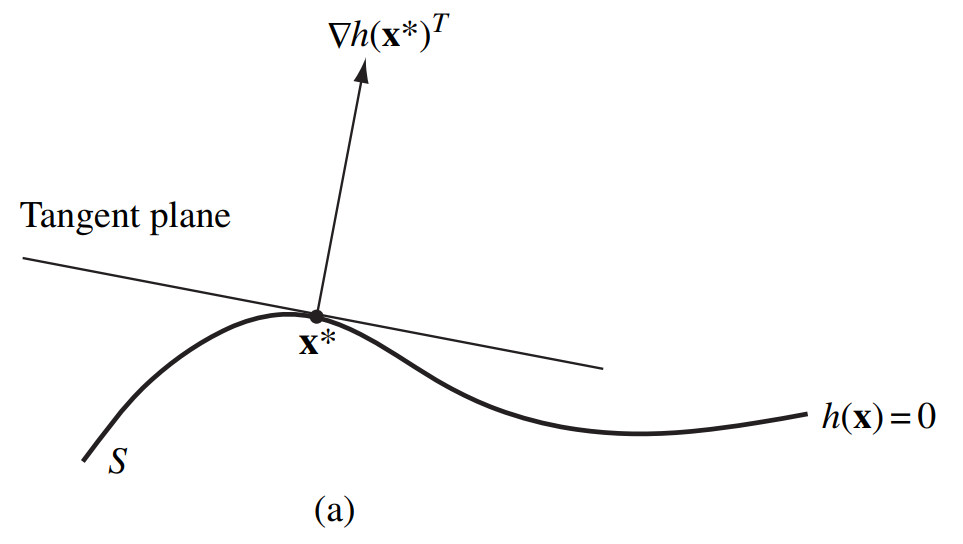
\includegraphics[scale=0.4]{Figures/duality/tan-1dim.png}
\centering
    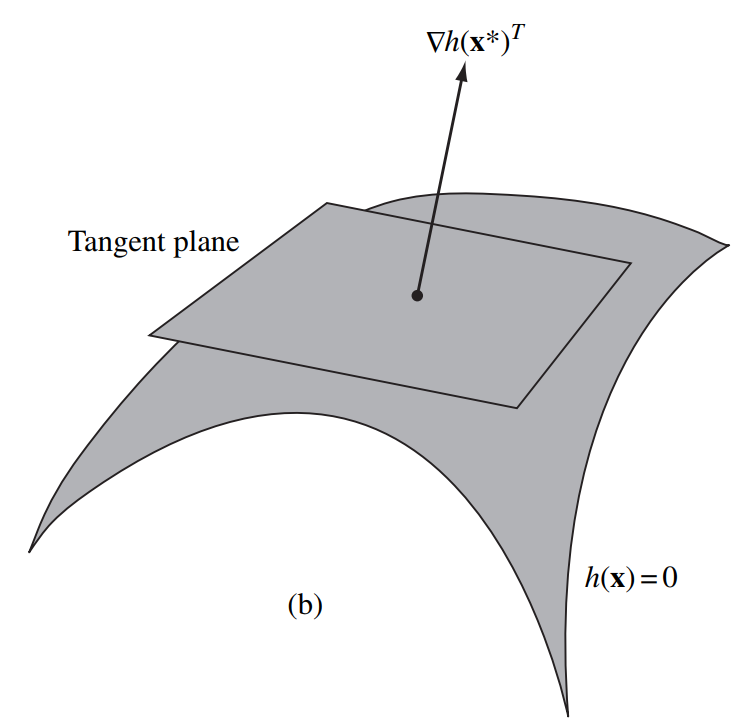
\includegraphics[scale=0.4]{Figures/duality/tan-2dim.png}
\caption{切空间的示意图}
\label{fig:tangent-space}
\end{figure}

对于\Cref{ex:tan-space},我们可以看到,
\[\nabla h_1(x)=(2x_1,2x_2,2x_3)\implies \nabla h_1(x^*)=(2,0,0).\]
因此,切空间$T_{x^*}(S^2)$的法向量是$(2,0,0)$,我们可以重新描述切空间为一个二维平面
\[T_{x^*}(S^2): 2x_1+0x_2+0x_3=0\iff x_1=0.\]
这和\Cref{ex:tan-space} 的结果是一致的.

记
\[M=\left\{\sum_{i} \alpha_i \nabla h_i(x^*)^\t:\alpha_i\in\R\right\},\]
即$M$是$\nabla h_i(x^*)^\t$张成的空间. 它的正交补是
\[M^\perp=\{{y}\in\R^n:\nabla {h(x^*)y}=0\},\]
这里,$\nabla {h(x^*)}$是$h$在$x^*$处的Jacobi矩阵\index{Jacobi矩阵},即对$h$的每一个分量求导得到的矩阵:
\[\nabla {h(x^*)}=\begin{pmatrix}
    \nabla h_1(x^*)\\
    \nabla h_2(x^*)\\
    \dots\\
    \nabla h_m(x^*)
\end{pmatrix}.\]

我们已经证明$T_{x^*}(S)\subseteq M^\perp$. 进一步,\Cref{ex:tan-space} 的结果表明,$T_{x^*}(S)=M^\perp$,即切空间和$M^\perp$是相等的. 然而,如果对于\Cref{ex:3d-constraint-2} 中的第一个$h$,我们会发现切空间和$M^\perp$是不相等的:$h(x)=0$对应的是单个点,对于单个点的切空间自然是一个零维空间,然而,和$\nabla h(x^*)$正交的空间是整个二维空间!

以上例子说明两件事,首先,切空间和$M^\perp$不一定相等;其次,切空间和$M^\perp$的关系和曲面的维度有关. 为了说明这一点,我们引入\emph{正规点}的概念. 

\begin{definition}[正规点]\label{def:regular-point}\index{正规点}
考虑优化问题 \eqref{eq:eq-constraint-only-differentiable},当一个点$x^*\in\Omega$满足约束${h(x^*)}=0$,且梯度向量$\nabla h_1(x^*),\nabla h_2(x^*),\dots,\nabla h_m(x^*)$线性无关时,它被称作该约束的\textbf{正规点}. 
\end{definition}

直观上来说,正规点上每一条约束都起到了实际的作用,因此梯度向量$\nabla h_i(x^*)$形成了一个线性无关的集合,张成了空间$M$. 此时,切空间恰好完全垂直于$M$,即$T_{x^*}(S)=M^\perp$. 这一几何直观见\Cref{fig:tan-2constraint},点${x^* }$处的两个等式约束共同确定了该点的切空间.
\begin{figure}
    \centering
    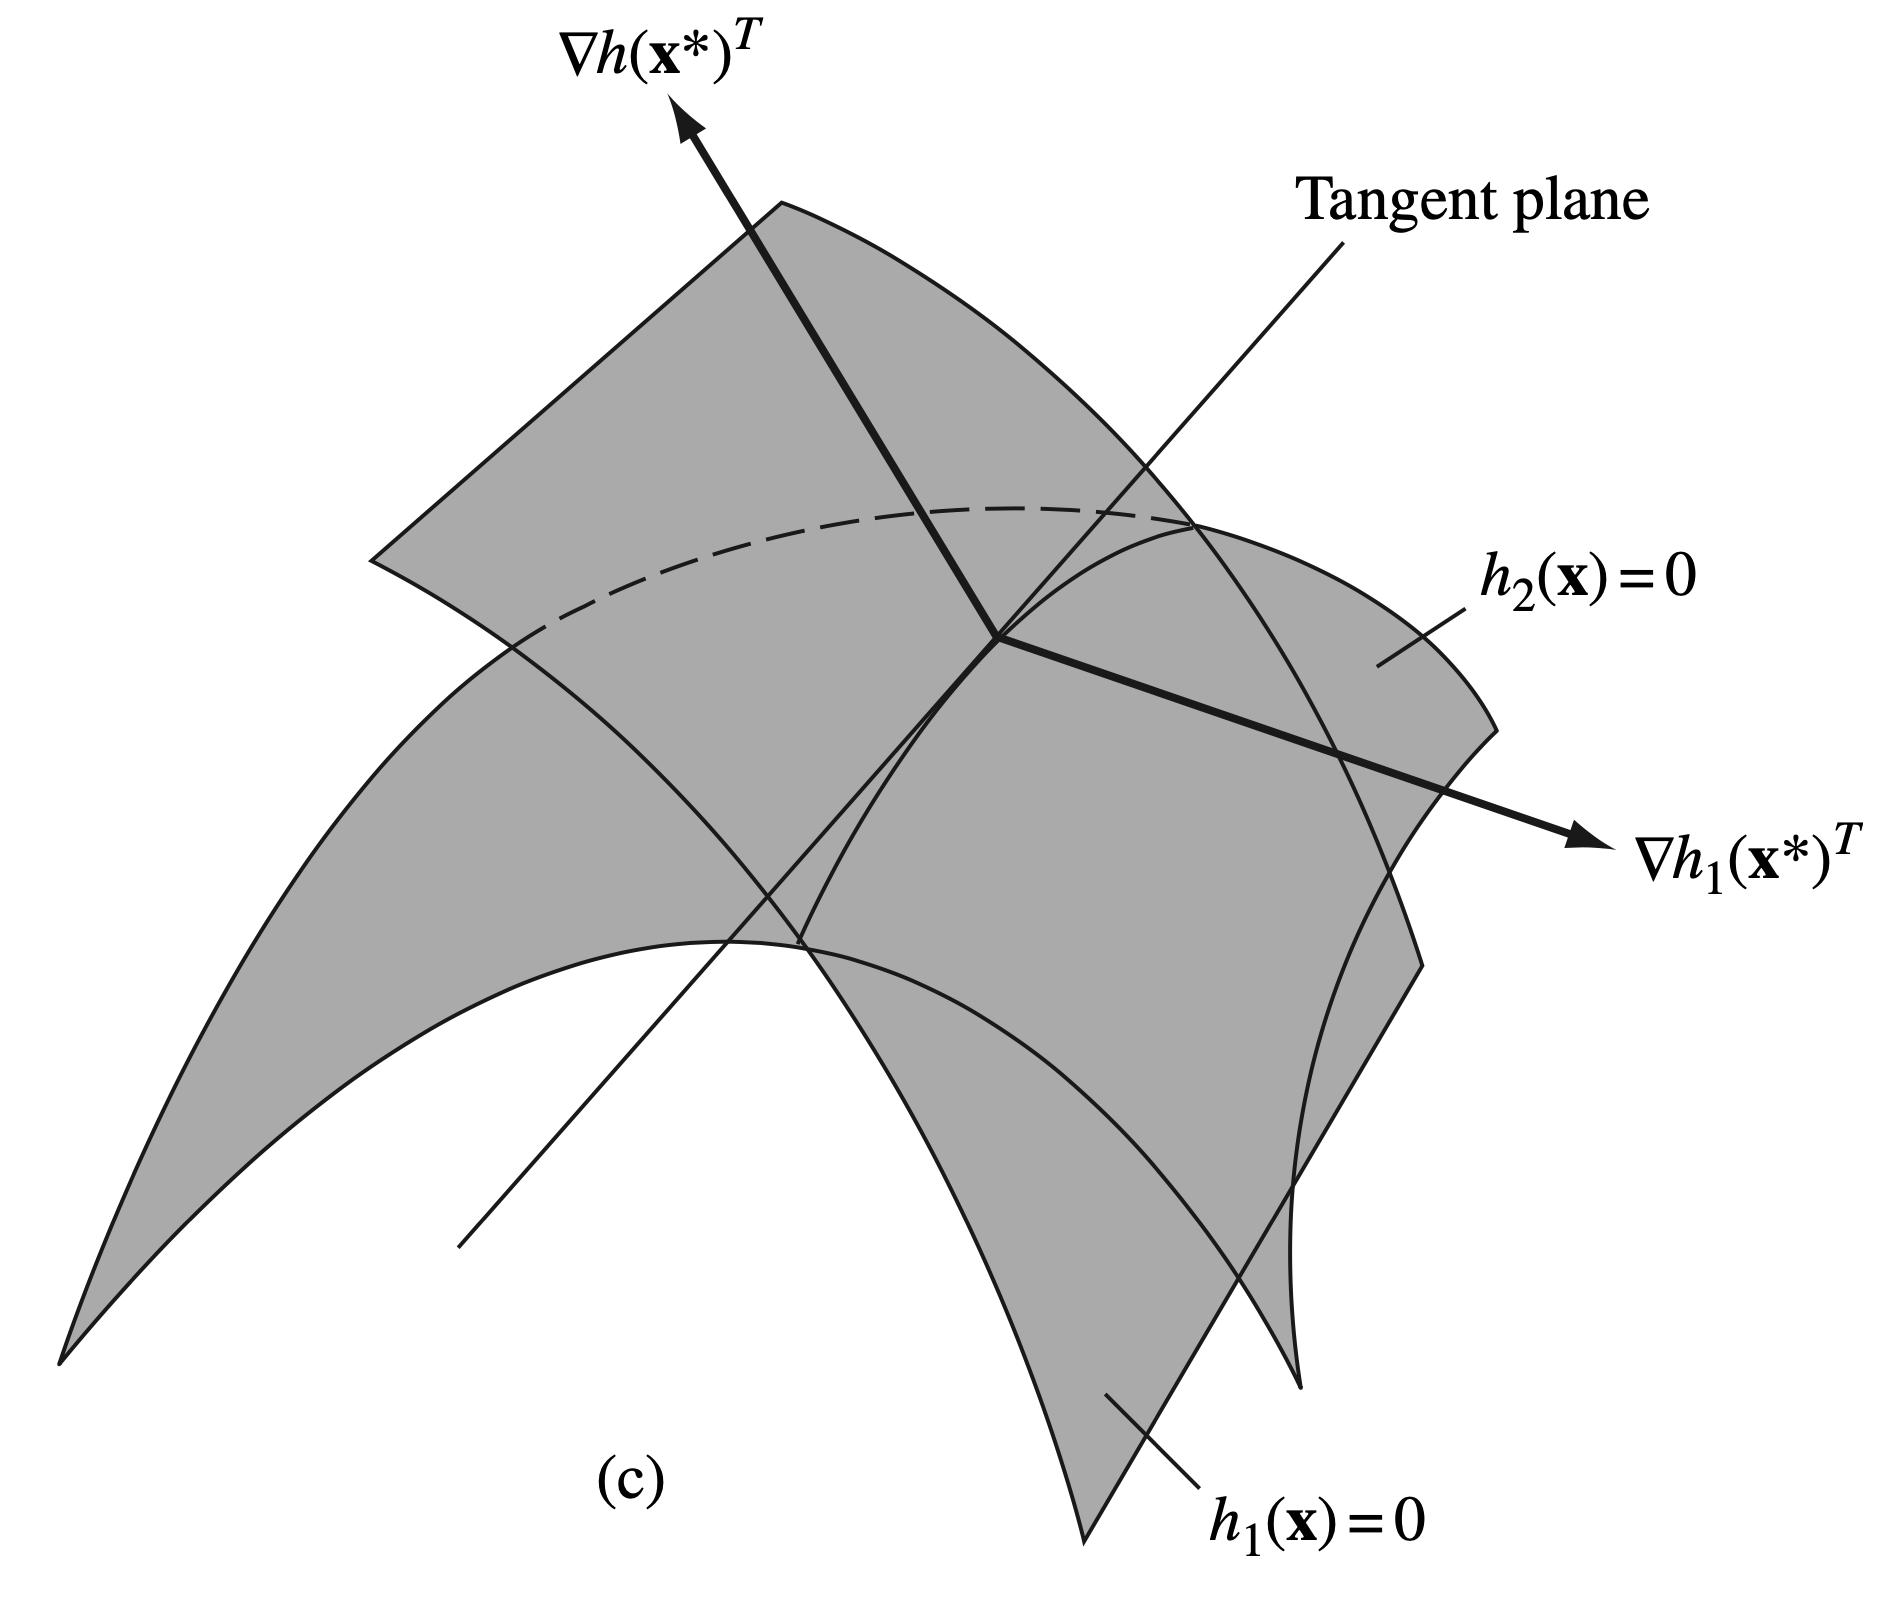
\includegraphics[scale=0.17]{Figures/duality/tan-2constraint.png}
    \caption{正规点示意图}
    \label{fig:tan-2constraint}
\end{figure}

\begin{theorem}[正规点切空间刻画定理]\label{thm:tan-space-characterize}\index{正规点切空间刻画定理}
设曲面$S\subseteq\R^n$由约束$h(x)=0$定义,$x^*\in S$是正规点,那么,
\[T_{x^*}(S)=M^\perp=\{{y:\nabla h(x^*)y=0}\}.\]
\end{theorem}
该定理的证明需要隐函数定理,对微积分要求较高,我们这里略去.

如此,针对正规点,我们找到了表达切空间的一种方法. 这一方法还揭示了曲面维度和约束的梯度向量的关系.

\begin{remark}
    实际上,梯度向量$\nabla h_i(x^*)$张成空间$M$的维数定义了曲面$S$在点$x^*$的维数. 如果在点$x^*\in S$一个邻域内维数都是$k$,那么,我们可以用一个$k$维的参数来描述这个邻域内的点. 这一性质被称为\emph{秩定理}\index{秩定理}.
\end{remark}

\section{条件极值与Lagrange乘子法}

有了切空间的准备,现在我们要对正规点推导带约束的优化问题的极值条件. 我们首先考虑只有等式约束的情况:

\begin{equation}
\begin{aligned}
\min\quad& f(x) \\
\text{s.t.}\quad& {h}(x)={0},\\
& x \in \Omega.
\end{aligned}    \label{eq:eq-constraint-only-differentiable}
\end{equation}
其中$f,h$都具有连续的一阶导数.

设$x^*$ 是一个约束$h(x)=0$一个正规点,同时也是函数$f$的一个在可行域中的极值点. 这一部分的目标是得到条件极值的一阶必要条件:
\begin{theorem}[条件极值的一阶必要条件]\label{thm:eq-opt-cond-1}\index{一阶必要条件}
    令$x^*$是一个$f$的满足约束${h(x)=0}$的正规极值点. 那么存在一个${\lambda}\in \R^m$使得$$\nabla f(x^*)+{\lambda^\t \nabla h(x^*)=0}. $$
\end{theorem}

一阶必要条件$\nabla f(x^*)+{\lambda^\t}\nabla {h(x^*)=0}$以及约束${h(x^*)=0}$给出了$n+m$个等式以及包含${x^*,\lambda}$在内的$n+m$个变量. 因此在非退化的情况下,他们给出了一个唯一解. 

引入与这个约束问题对应的Lagrange函数:
        $$l({x,\lambda})=f(x)+{\lambda^\t h(x)}.$$
$\lambda$被称为\emph{Lagrange乘子}\index{Lagrange乘子}. 必要条件可以被写作:
\begin{align*}
    \nabla_x l({x,\lambda})&=0,\\
    \nabla_{\lambda} l({x,\lambda})&=0.
\end{align*}

这一个求解条件极值的方法会在大部分微积分课程中给出,我们这里的更重要的任务是给出这一方法的几何解释. 注意,\Cref{thm:eq-opt-cond-1} 本质上在说,$\nabla f(x^*)$是$\nabla h_i(x^*)$的线性组合,所以我们的目标就是得到这一事实。

假设$h(x)=0$形成的曲面是$S$,考虑正规极值点$x^*\in S$. 我们任选一条曲线$x(t)$过$x^*=x(0.5)$,那么,$f(x(t))$在$t=0.5$处取得了极小值. 根据微积分的极值定理,我们有
\[\left.\frac{\d}{\d t}f(x(t))\right|_{t=0.5}=0\iff \nabla f(x^*)\dot{x}(0.5)=0.\]
因此,$\nabla f(x^*)$和切向量$\dot{x}(0.5)$正交,因为曲线$x(t)$是任意选取的,所以$\nabla f(x^*)$也和切空间$T_{x^*}(S)$正交.

现在,回忆\Cref{thm:tan-space-characterize},我们知道切空间$T_{x^*}(S)=M^\perp$,因此
\[\nabla f(x^*)^\t\in (M^\perp)^\perp=M=\left\{\sum_{i} \lambda_i \nabla h_i(x^*)^\t:\lambda_i\in\R\right\}.\]
换言之,$\nabla f(x^*)$是$\nabla h_i(x^*)$的线性组合,这就证明了\Cref{thm:eq-opt-cond-1}.


最后,作为应用,我们考虑一个例子.

\begin{example}[最大熵]\label{ex:max-entropy}
考虑一个离散的概率分布,其分布列为$p_i=\Pr(X=x_i),i=1,\dots,n$. 该分布的熵为
$$\epsilon = -\sum_{i=1}^n p_i \log p_i.$$
该分布的均值为$\sum_{i=1}^n x_i p_i$. 

如果均值固定为$m$,求解使熵最大化的参数可以被转化成以下问题:
\begin{align*}
\max\quad&-\sum_{i=1}^n p_i\log p_i \\
\text{s.t.}\quad& \sum_{i=1}^n p_i=1, \\
&\sum_{i=1}^n x_i p_i=m, \\
&p_i\geq 0, \qquad i=1,2,\dots,n.
\end{align*}

我们先忽略非负约束,假设这些约束不会被触发. 引入两个Lagrange乘子,$\lambda$和$\mu$,则Lagrange函数为
$$l=\sum_{i=1}^n (-p_i\log p_i+\lambda p_i+\mu x_ip_i)-\lambda-\mu m.$$
由一阶必要条件,$-\log p_i -1+\lambda+\mu x_i=0$,$i=1,2,\dots,n$. 因此,
$$p_i=\exp((\lambda-1)+\mu x_i),\quad i=1,2,\dots, n.$$
注意$p_i>0$,所以非负约束确实没有被触发. Lagrange乘子$\lambda$和$\mu$是两个用来保证等式约束被满足的参数. 
\end{example}

\section{Karush–Kuhn–Tucker条件}
现在加入不等式约束,考虑以下形式的问题:
\begin{equation}
\begin{aligned}
\min\quad& f(x) \\
\text{s.t.}\quad& h(x)=0, \\
&g(x)\leq 0,\\
& x \in \Omega.
\end{aligned}\label{eq:ineq-constraint-inequality-differentiable}
\end{equation}
其中$f,h,g$具有连续的一阶导数。

我们将使用Lagrange乘子法来推导一阶必要条件. 现在,最主要的问题在于多了不等式约束,我们需要找到一种方法来处理这些约束.

假设$x^*$是一个极小值点,那么,我们可以将不等式约束$g(x)\leq 0$分为两部分:
\begin{itemize}
    \item $g_i(x^*)<0$。根据$g_i$的连续性,在$x^*$的一个邻域内,恒有$g_i(x)<0$,因此这个约束在$x^*$附近一定不会违背。我们称这样的约束为\emph{非激活约束}\index{非激活约束}.
    \item $g_i(x^*)=0$。如果稍微偏离$x^*$,那么$g_i(x)$可能会变成正数,因此,这个约束在$x^*$附近是起作用的. 我们称这样的约束为\emph{激活约束}\index{激活约束}.
\end{itemize}

因此,在$x^*$的一个邻域$U$内,如果激活的约束下标集是$J$,那么 \eqref{eq:ineq-constraint-inequality-differentiable} 可以被写作:
\begin{equation}
\begin{aligned}
    \min\quad& f(x) \\
    \text{s.t.}\quad& h(x)=0, \\
    &g_i(x)=0, \quad i\in J,\\
    & x \in U.
\end{aligned}
\label{eq:ineq-constraint-inequality-differentiable-active}
\end{equation}

根据这一观察,我们可以自然地推广正规点$x^*$的定义:
\begin{definition}[正规点]\index{正规点}
考虑优化问题 \eqref{eq:ineq-constraint-inequality-differentiable},如果一个点$x^*$满足以下条件:
\begin{itemize}
    \item 它是可行域中的点:$h(x^*)=0$,$g(x^*)\leq 0$,$x\in\Omega$,
    \item 令$J$为满足$g_j(x^*)=0$的下标$j$的集合(激活的约束). 那么,梯度向量$\nabla h_i(x^*)$,$\nabla g_j(x^*)$,$1\leq i \leq m$,$j\in J$是线性无关的,
\end{itemize}
那么,$x^*$被称作该约束的\textbf{正规点}.
\end{definition}

换言之,此时的正规点不仅考虑等式约束,还要考虑起作用的(被激活的)不等式约束,这些不等式约束相当于等式约束. 类似Lagrange乘子法,此时的一阶必要条件为:

\begin{theorem}[Karush-Kuhn-Tucker条件]\label{thm:KKT}\index{Karush-Kuhn-Tucker条件}\index{一阶必要条件}
令$x^*$为优化问题 \eqref{eq:ineq-constraint-inequality-differentiable} 的正规极小值点,那么,存在向量$\lambda\in\R^m$和向量$\mu\in \R^p$且$\mu\geq 0$使得
\begin{align}
    \nabla f(x^*)+\lambda^\t \nabla {h(x^*)}+\mu^\t \nabla g(x^*)&=0,\label{eq:KKT-1}\\
    {\mu^\t g(x^*)}&=0.\label{eq:KKT-2}
\end{align}
\end{theorem}

\begin{proof}
考虑$x^*$的邻域$U$,在这个邻域内,我们可以将问题 \eqref{eq:ineq-constraint-inequality-differentiable} 写作 \eqref{eq:ineq-constraint-inequality-differentiable-active},即只考虑激活的约束. 由于$x^*$是一个极小值点,根据\Cref{thm:eq-opt-cond-1},存在$\lambda\in\R^m,\mu\in\R^p$使得
\[
\nabla f(x^*)+\lambda^\t \nabla {h(x^*)}+\mu_J^\t \nabla g_J(x^*)=0.
\]
这里,$\nabla g_J(x^*)=(\nabla g_j(x^*))_{j\in J}$,即只考虑激活的约束.

对于非激活的下标$i$,我们补充定义$\mu_i=0$,于是,上式可以被写作
\[\nabla f(x^*)+\lambda^\t \nabla {h(x^*)}+\mu^\t \nabla g(x^*)=0.\]
这就得到了 \eqref{eq:KKT-1}.

对于被激活的下标$i$,我们有$g_i(x^*)=0$,因此,$\mu_i g_i(x^*)=0$;对于非激活的下标$i$,我们有$\mu_i=0$,因此,$\mu_i g_i(x^*)=0$. 于是,\eqref{eq:KKT-2} 得证.

最后,我们还需要证明$\mu\geq 0$. 因为$x^*$是\emph{可行域}内的极小值,所以,假设$x^*$沿着方向$y$使得恰好有一个$g_k$从激活变为非激活,因为此时还在可行域,$f$应该不变小。

下面我们来选取这样的$y$. 考虑如下曲面:
\[S=\{x\in\R^n:h(x)=0,g_j(x)=0, j\in J\setminus\{k\}\}.\]
也就是除了$k$之外所有的等式约束形成的曲面. 我们从切空间$T_{x^*}(S)$中选取一个$y$,使得$\nabla g_k(x^*)y<0$,这样,$g_k$会从激活变为非激活,而其他约束依然得到满足。这一选择的几何示意如\Cref{???} \lhysays{补个图} 所示。

下面我们说明为什么这样的$y$存在。因为$x^*$是正规点,所以根据\Cref{thm:tan-space-characterize},$T_{x^*}(S)=M^\perp$,其中

\[M=\left\{\sum_{i} \alpha_i \nabla h_i(x^*)^\t+\sum_{j\in J\setminus\{k\}} \beta_j \nabla g_j(x^*)^\t:\alpha_i,\beta_j\in\R\right\}.\]
根据正规点的定义,$\nabla g_k(x^*)^\t$不在$M$中,所以,$\nabla g_k(x^*)^\t$在$M^\perp$中的分量非零,于是,我们可以选择一个$y\in M^\perp$使得$\nabla g_k(x^*)y<0$。

将$y$右乘 \eqref{eq:KKT-1},我们有
\[\nabla f(x^*)y+\lambda^\t \nabla h(x^*)y+\mu^\t \nabla g(x^*)y=0.\]
这等价于
\[\nabla f(x^*)y+\mu_k\nabla g_k(x^*)y=0.\]
令$x(t)$为一条在$S$内且经过$x^*$(此处$t=0$)的曲线,且有$\dot{x}(0)={y}$. 根据极小值的定义
\begin{align*}
    &0\leq \left.\frac{\d f(x(t))}{\d t}\right|_{t=0}=\nabla f(x^*)y=-\mu_k\underbrace{\nabla g_k(x^*)y}_{<0}.\\
    \iff&\mu_k\geq 0.
\end{align*}
这一证明对所有激活约束的$k$都成立,所以这就完成了证明。
\end{proof}

条件 \eqref{eq:KKT-1} 对应的就是Langrange乘子,而 \eqref{eq:KKT-2} 则是\emph{互补松弛条件}\index{互补松弛条件}:

\begin{proposition}[互补松弛条件]
    对于一个优化问题 \eqref{eq:ineq-constraint-inequality-differentiable},考虑一个正规极小值点$x^*$和对应的Lagrange乘子$\lambda,\mu$。我们有以下结论:
    \begin{itemize}
        \item $\mu\geq 0$;
        \item 如果$g_i(x^*)<0$,那么$\mu_i=0$;
        \item 如果$\mu_i>0$,那么$g_i(x^*)=0$.
    \end{itemize}
\end{proposition}

下面我们来看一个运用KKT条件的例子:
\begin{example}
考虑问题
\begin{align*}
    \min \quad &2x_1^2+2x_1x_2+x_2^2-10x_1-10x_2 \\
    \text{s.t.}\quad &x_1^2+x_2^2\leq 5, \\
    & 3x_1+x_2\leq 6.
\end{align*}
KKT条件为
\begin{align*}
    4x_1+2x_2-10+2\mu_1x_1+3\mu_2&=0, \\
    2x_1+2x_2-10+2\mu_1x_2+\mu_2&=0, \\
    \mu_1(x_1^2+x_2^2-5)&=0, \\
    \mu_2(3x_1+x_2-6)&=0,\\
    \mu_i&\geq 0,\quad i=1,2.
\end{align*}
为了求解此类问题,我们假设一些约束被激活,然后检查所得出的Lagrange乘子的符号正负. 在这个问题中,我们可以尝试假设有0,1,2个约束被激活. 

假设第一个约束被激活,第二个约束没有被激活,得出等式
\begin{align*}
4x_1+2x_2-10+2\mu_1x_1&=0, \\
2x_1+2x_2-10+2\mu_1x_2&=0, \\
x_1^2+x_2^2&=5.
\end{align*}
可得解$x_1=1,x_2=2,\mu_1=1.$

由于$3x_1+x_2=5$,因此第二个约束也被满足了. 因此,因为$\mu_1 > 0$,我们得出结论,这个解满足一阶必要条件. 
\end{example}

\section{Lagrange对偶}
\subsection{Lagrange定理}
现在,我们不再假设函数可微,我们考虑极值点的零阶必要条件\index{零阶必要条件},首先考虑只有等式约束的情形:
    \begin{equation}
          \begin{aligned}
        \min&\quad f(x) \\
        \text{s.t.}\quad& {h(x)=0}, \\
        &x\in\Omega.
        \end{aligned}\label{eq:eq-zero-cond}
    \end{equation}
如果函数$f$是凸函数,$m$维函数${h}$是仿射的,并且集合$\Omega\subseteq \R^n$是是凸的,那么这个规划问题是一个\emph{凸规划问题}\index{凸规划问题}. 

为了给这样的问题一个一阶必要条件,我们依然需要引入正规性条件. 此时正规性不再仅仅只对一个点,而是对仿射函数$h$.

\begin{definition}[正规性条件]\index{正规性条件}
一个仿射函数${h}$关于集合$\Omega$是\textbf{正规的},指的是像集$h(\Omega)=\{y:\exists x\in\Omega\ h(x)=y\}$包含${0}$处的一个开球邻域. 也就是说,$h(\Omega)$包含一个形如$\{y:\norm{y}<\epsilon\}$(对某个$\epsilon>0$)的集合. 
\end{definition}

\begin{remark}
这个条件是一阶正规点定义的推广. 如果${h}$在点$x^*$有连续的导数,那么一阶正规性条件意味着$\nabla{h(x^*)}$是满秩的,并且由隐函数定理可知存在一个$\epsilon>0$使得对于任意满足${\norm{y-h(x^*)}}<\epsilon$的${y}$,都有一个$x$使得${h(x)=y}$. 换言之,存在一个${y^*=h(x^*)}$周围的开球.
\end{remark}

我们可以用Lagrange乘子来表述零阶必要条件:
\begin{theorem}[零阶必要条件,等式约束情形]\label{thm:eq-zero-cond}\index{零阶必要条件}
假设$\Omega\subseteq\R^n$是凸的,$f$是$\Omega$上的凸函数,${h}$是一个$\Omega$上的$m$维仿射函数. 假设${h}$是对于$\Omega$正规的. 如果$x^*$是 \eqref{eq:eq-zero-cond} 的解,那么存在${\lambda}\in \R^m$使得$x^*$是以下Lagrange问题的解:\begin{align*}
    \min\quad& f(x)+{\lambda^\t h(x)}\\
    \text{s.t.}\quad & x\in\Omega.
\end{align*}
\end{theorem}

这一定理证明的关键在于引入\emph{原始函数}. 对应于问题\eqref{eq:eq-zero-cond} 的\textbf{原始函数}\index{原始函数}是:$$\omega({y})=\inf\{f(x):{h(x)=y,x}\in\Omega\},\quad y\in h(\Omega).$$


\begin{proof}[零阶必要条件的证明]
令$f^*=f(x^*)$. 定义$\R^m\times\R$内的集合$A$和$B$为:
\begin{align*}
    A&=\{(y,r):r\geq \omega({y}),{y}\in h(\Omega)\},\\ 
    B&=\{(y,r):r\leq f^*,y=0\}.
\end{align*}
$A$是$\omega$的上图,$B$是$f^*$向下延申并与原点对齐的垂线. $A$和$B$都是凸集. 他们唯一的公共点是$(0,f^*)$. 由超平面分离定理可知,存在一个超平面分离$A$和$B$. 这个超平面可以被表示成一个在$\R^m\times\R$内的形如$(\lambda,s),\lambda\in \R^{m}$的非零向量,还有一个分离常数$c$. 分离条件是$$sr+{\lambda^\t y}\geq c,\quad\forall(y,r)\in A,\quad sr+{\lambda^\t y}\leq c,\quad\forall(y,r)\in B.$$ 
这一过程的示意图见\Cref{fig:sep-hyperplane-eq}.

\begin{figure}[ht]
    \centering
    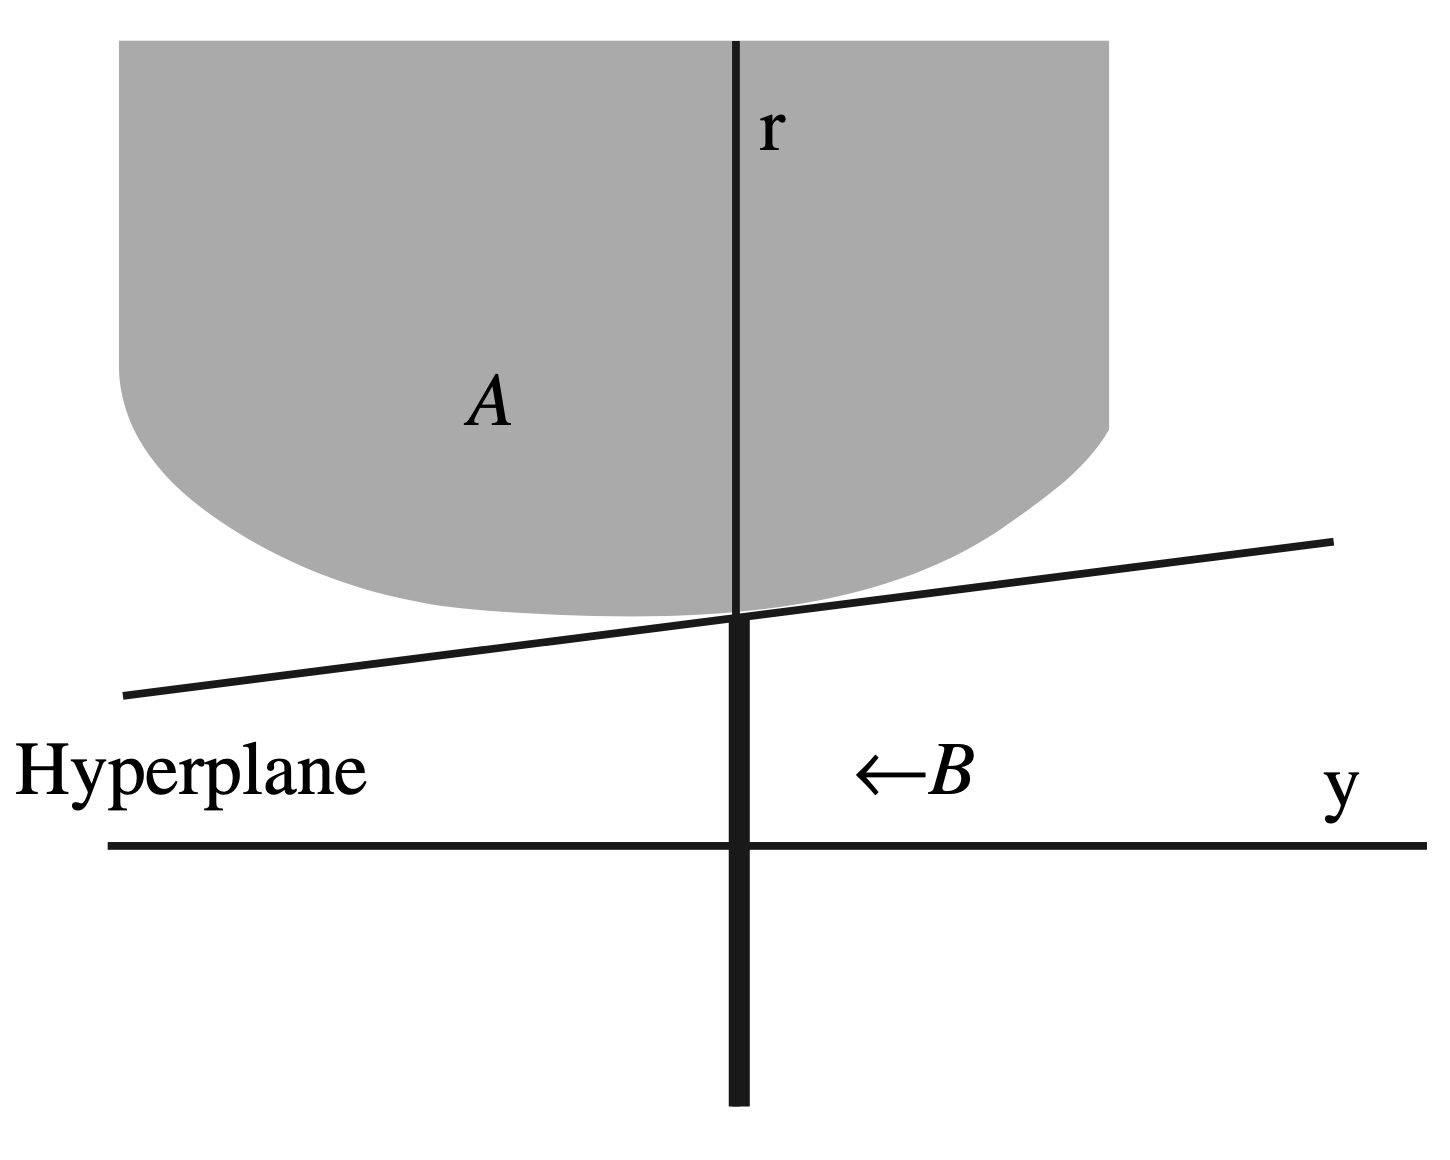
\includegraphics[scale=0.3]{Figures/duality/sep-hyperplane-eq.png}
    \caption{证明示意图. }
    \label{fig:sep-hyperplane-eq}
\end{figure}

注意到$s\geq 0$,否则取$|r|$非常大的负数$r$,点$(r,{0})\in B$违反第二个分离不等式. 几何上看,若$s=0$,超平面将垂直. 我们来证明$s\neq 0$. 假设$s=0$,因为$s$和${\lambda}$不能都是$0$,${\lambda\neq 0}$. 因为分离超平面必须包含点$(f^*,{0})$,从第二个分离不等式得$c=0$. 由$h$的正规性,以${0\in h(\Omega)}$为中心的某个球包含在$h(\Omega)$中,任取$y$属于这个开球. 第一个分离不等式左侧为${\lambda^\t y}$,它对于某些${y}$来说是负的. 这违背第一个分离不等式. 因此$s\neq 0$,继而$s>0$. 

不失一般性,可以假设$s=1$. 假设$x\in\Omega$. 那么$(h(x),f(x))\in A$且$(0,f(x^*))\in B$. 因此,由分离不等式可知,我们有$$f(x)+{\lambda^\t h(x)}\geq f(x^*)=f(x^*)+{\lambda^\t h(x^*)}.$$ 因此$x^*$是优化问题 \eqref{eq:eq-zero-cond} 解. 
\end{proof}

我们再考虑只有不等式约束的模型
\begin{equation}
    \begin{aligned}
    \min\quad & f(x)\\
    \text{s.t.}\quad& {g(x)\leq 0},\\
    &x\in\Omega.
\end{aligned}\label{eq:ineq-zero-cond}
\end{equation}
其中,${g}$是一个$p$维的函数. 


然后我们引入正规性条件. 对于不等式约束来说,正规性条件也被称为做\emph{Slater条件}. 

\begin{definition}[Slater条件]\index{正规性条件}\index{Slater条件}
考虑优化问题 \eqref{eq:ineq-zero-cond},令
\[D=\{z\in \R^p:\exists x\in\Omega\ {g(x)\leq z}\}.\]
正规性条件(Slater条件)为:存在一个$z^\prime\in D$使得$z^\prime<0$. 
\end{definition}
直观来说,Slater条件指的是存在满足约束的内点.

类似地,我们可以用Lagrange乘子来表述零阶必要条件:
\begin{theorem}[零阶必要条件,不等式情形]\label{thm:ineq-zero-cond}\index{零阶必要条件}
假设$\Omega$是一个$\R^n$的凸子集,且$f$和${g}$是凸函数. 假设优化问题 \eqref{eq:ineq-zero-cond} 满足正规性条件,$x^*$是该问题的解,那么存在一个向量${\mu}\in \R^p$满足$\mu\geq 0$使得$x^*$是下述Lagrange问题的解:
\begin{align*}
\min\quad &f(x^*)+\mu^\t g(x)\\
\text{s.t.}\quad& x\in\Omega.
\end{align*}
此外,${\mu^\t g(x^*)}=0.$
\end{theorem}

这一定理的证明类似于\Cref{thm:eq-zero-cond} 的证明. 首先还是引入原始函数. 问题 \eqref{eq:ineq-zero-cond} 对应的原始函数\index{原始函数}为:
    $$\omega({z})=\inf\{f(x):g(x)\le{z},x\in\Omega\},z\in D.$$


\begin{proof}[证明概要]
令$f^*=f(x^*)$. 在$\R^{p}\times\R$内定义两个集合
\begin{align*}
    A&=\{(z,r):r\geq \omega(z), z\in D\},\\
    B&=\{(z,r):r\leq f^*, z\leq 0\}.
\end{align*}
$A$和$B$都是凸的. 证明依然是构造$A,B$的分离超平面,正规性条件保证了超平面不会是垂直的. 这个过程的示意见图\Cref{fig:sep-hyperplane-ineq}.
\begin{figure}
    \centering
    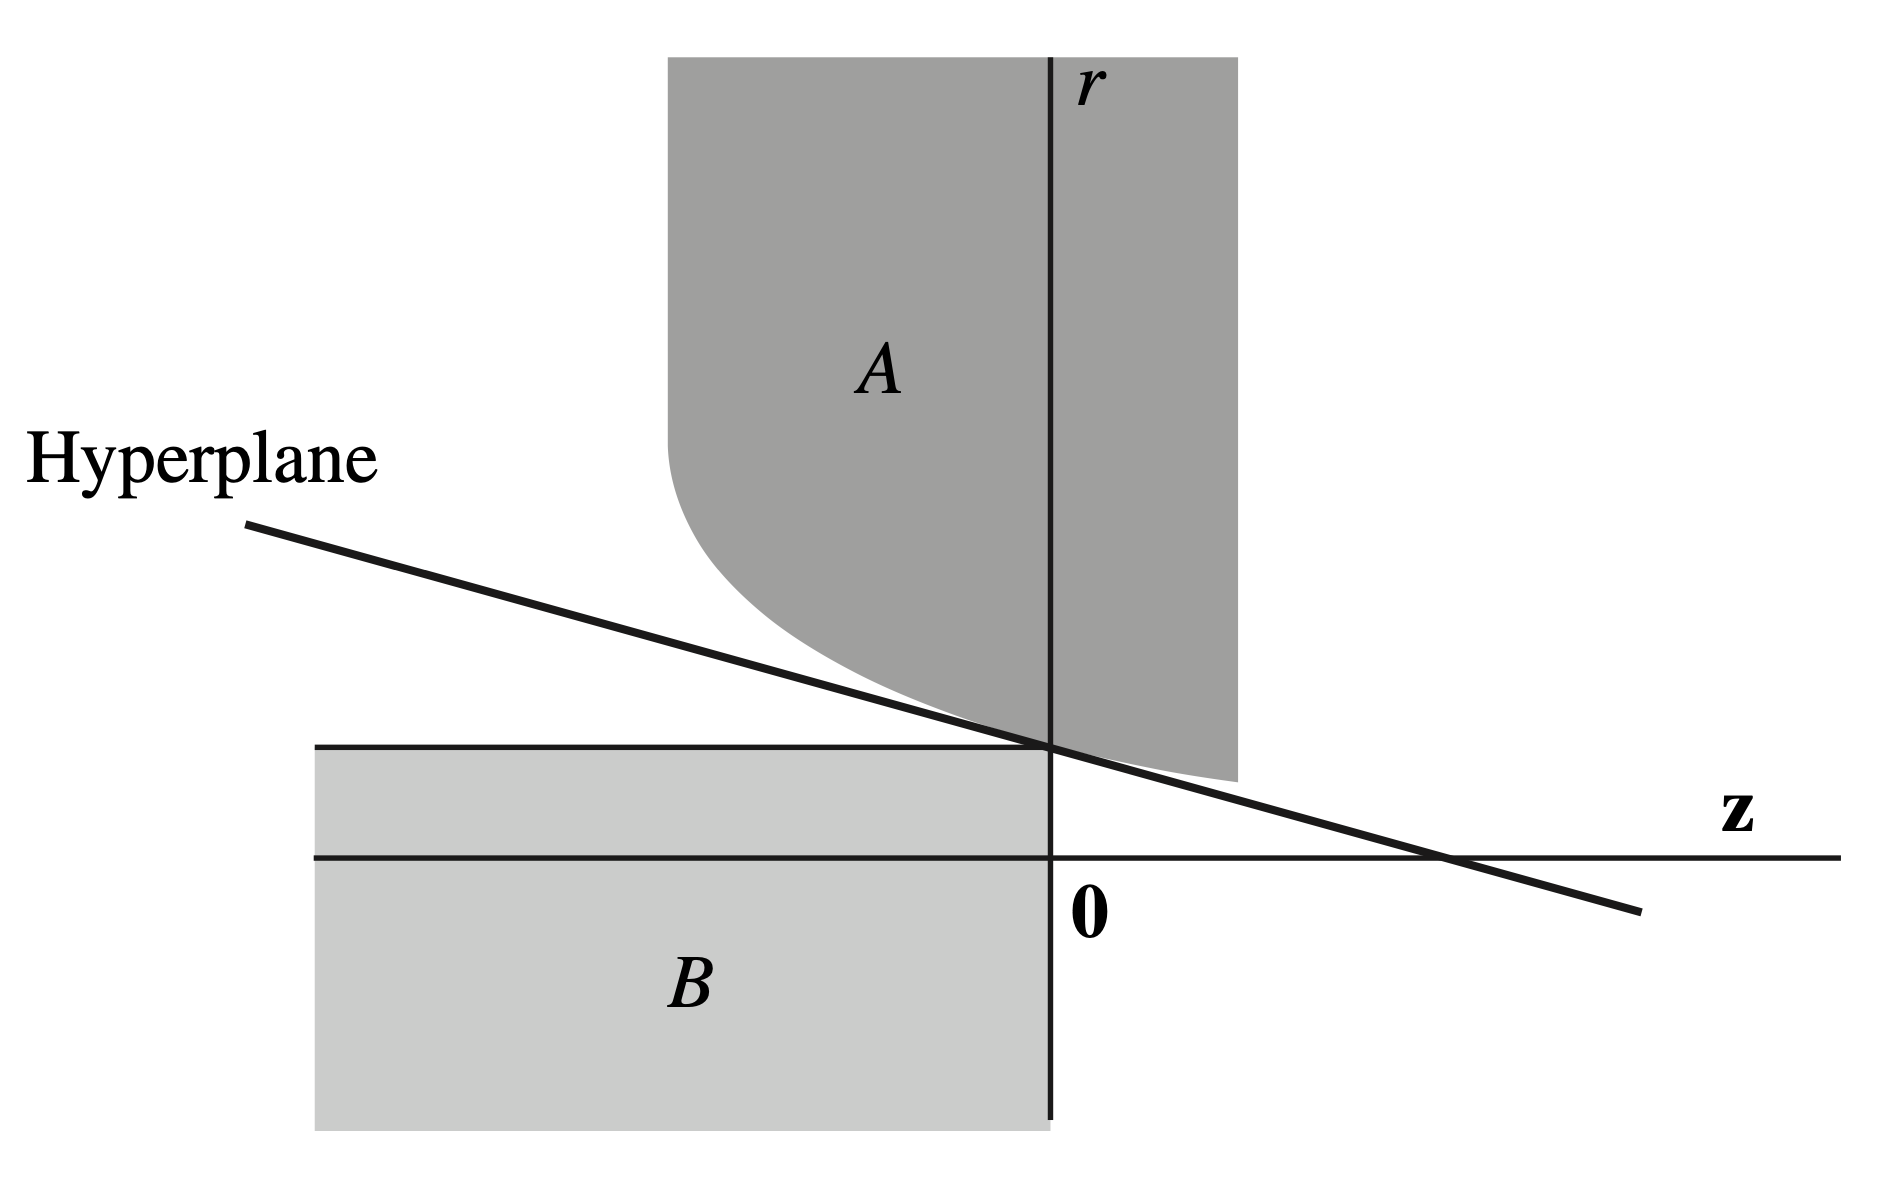
\includegraphics[scale=0.3]{Figures/duality/sep-hyperplane-ineq.png}
    \caption{证明示意图. }
    \label{fig:sep-hyperplane-ineq}
\end{figure}

条件$\mu^\t g(x^*)=0$是互补松弛条件,这一讨论类似KKT条件. 
\end{proof}

现在,我们考虑一般情形,
    \begin{equation}
          \begin{aligned}
        \min\quad & f(x) \\
        \text{s.t.}\quad& {h(x)=0}, \\
        &g(x)\leq 0, \\
        &x\in\Omega.
        \end{aligned}\label{eq:mix-zero-cond}
    \end{equation}
组合以上两个零阶必要条件,我们得到一般情形的Lagrange定理.

\begin{theorem}[Lagrange,零阶必要条件,混合情形]\label{thm:mix-zero-cond}\index{零阶必要条件}\index{Lagrange定理}
假设$\Omega\subseteq \R^n$是凸集. $f$和${g}$是一维和$p$维的凸函数,${h}$是维数为$m$的仿射函数. 假设${h}$满足对于$\Omega$的正规性条件,且$g$在 \eqref{eq:mix-zero-cond} 的可行域上满足正规性条件. 假设$x^*$是问题 \eqref{eq:mix-zero-cond} 的解. 那么存在向量${\lambda}\in \R^m$和${\mu}\in \R^p$满足${\mu}\geq {0}$使得$x^*$是以下Lagrange问题的解:
\begin{align*}
\min\quad &f(x)+\lambda^\t h(x)+\mu^\t g(x) \\
\text{s.t.}\quad& x\in\Omega.
\end{align*}
此外,${\mu^\t g(x^*)}=0.$
\end{theorem}

\lhysays{举个例子}


\subsection{弱对偶定理,强对偶定理}
Lagrange定理有非常强的几何直观,这一直观最终导致了优化中的\emph{对偶理论}\index{对偶理论}. 先考虑不等式约束的情形:
\begin{equation}
    \begin{aligned}
    \min\quad & f(x)\\
    \text{s.t.}\quad& {g(x)\leq 0},\\
    &x\in\Omega.
\end{aligned}\label{eq:ineq-dual}
\end{equation}
$\Omega\subseteq \R^n$是凸集,函数$f$和${g}$定义在$\Omega$上. 函数${g}$是$p$维的. 

回忆原始函数的定义:
        $$\omega({z})=\inf \{f(x):g(x)\leq z,x\in\Omega\}.$$

设$x^*$是 \eqref{eq:ineq-dual} 的解,$f^*=f(x^*)$,那么函数$\omega(z)$与纵轴的交点是$f^*$. 如果 \eqref{eq:ineq-dual} 没有解,那么$f^*=\inf\{f(x):g(x)\leq 0,x\in\Omega\}$就是纵轴与$\omega(z)$的交点. 考虑在$\omega(z)$以下的超平面,关注其纵截距(见图\Cref{fig:hyperplane-below}),我们用它产生对偶原理.
\begin{figure}
    \centering
    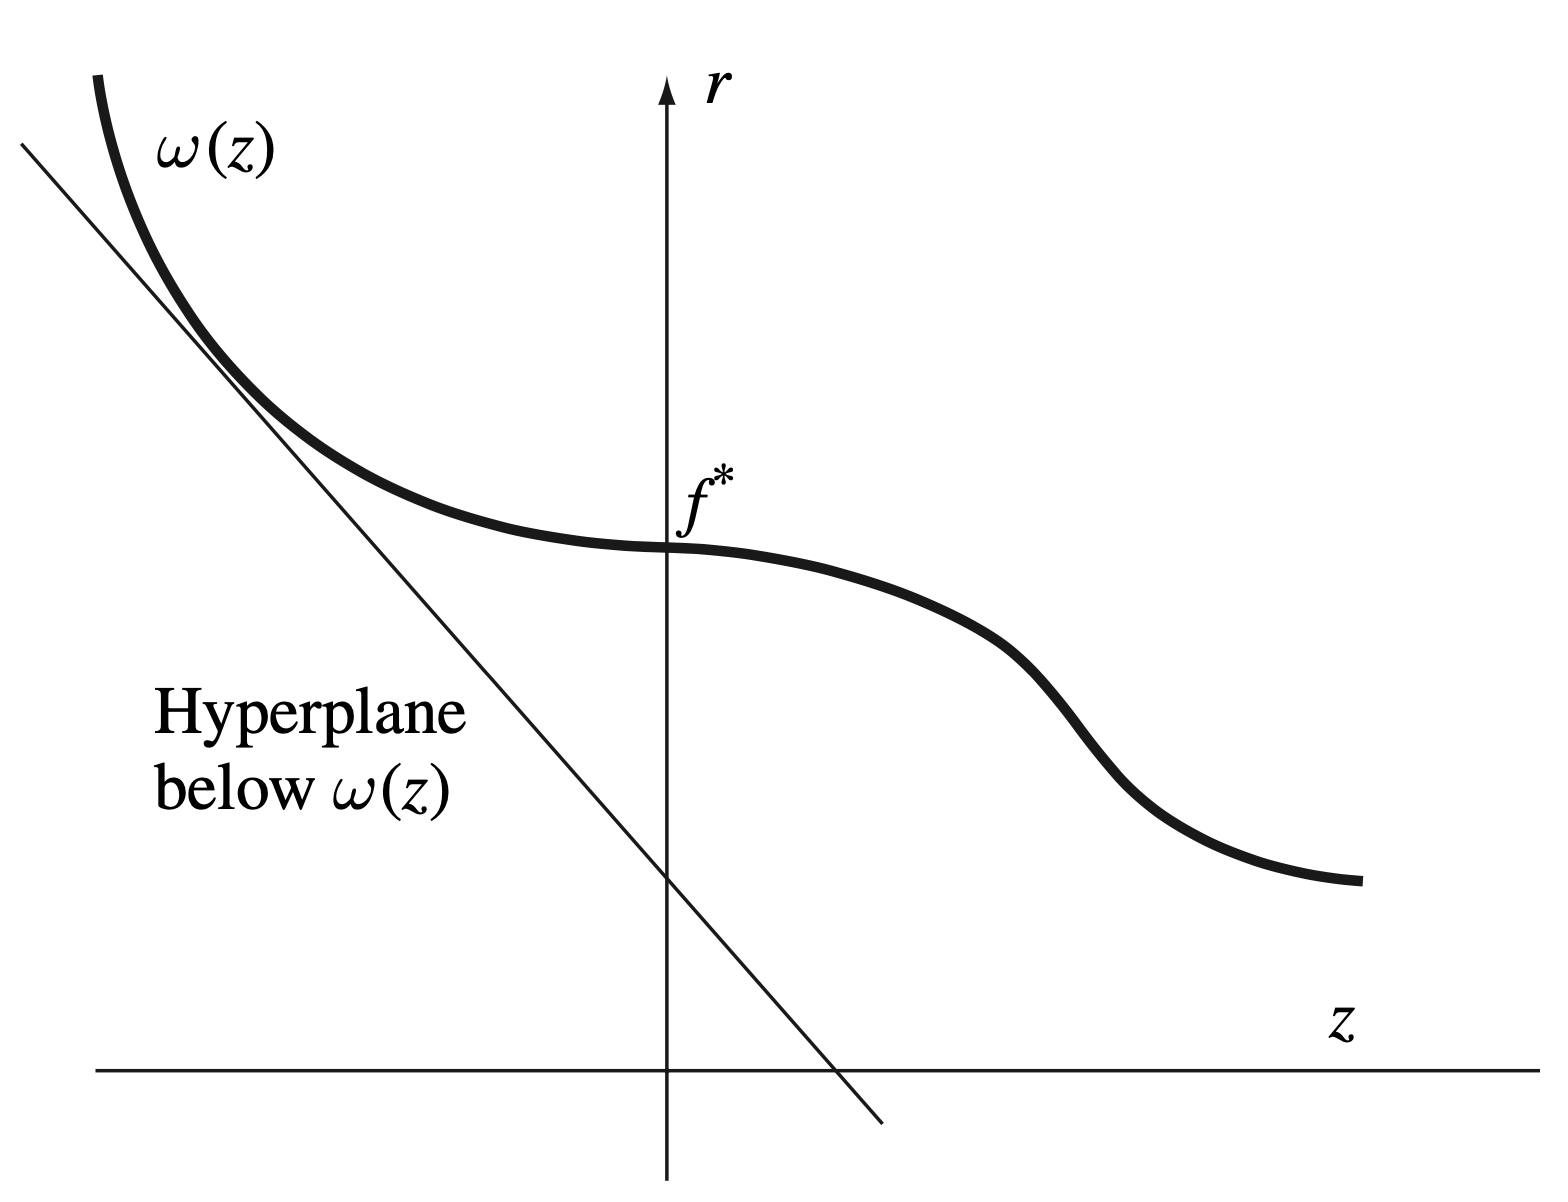
\includegraphics[scale=0.2]{Figures/duality/hyperplane-below.png}
    \caption{纵截距的示意图.}
    \label{fig:hyperplane-below}
\end{figure}

为了刻画超平面以及其纵截距,我们引入对偶函数. 在$\R^p_{\geq 0}$上定义\textbf{对偶函数}\index{对偶函数}为:
$$\varphi({\mu})=\inf \{f(x)+{\mu^\t g(x)}:x\in\Omega\}.$$
定义其最大值为
    \[\varphi^*=\sup\{\varphi(\mu),\mu\geq 0\}.\]

我们很容易可以证明以下定理:

\begin{theorem}[弱对偶定理]\label{thm:weak-dual}\index{弱对偶定理}
    $\varphi^*\leq f^*$.
\end{theorem}

\begin{proof}
    对任意${\mu \geq 0}$我们有
    \begin{align*}
        \varphi({\mu}) &=\inf\{f(x)+{\mu^\t g(x):x}\in\Omega\} \\
        & \leq \inf\{f(x)+{\mu^\t g(x):g(x)\leq 0,x}\in\Omega\} \\
        & \leq \inf\{f(x):{g(x)\leq 0, x}\in\Omega\}=f^*.
    \end{align*}
    由此,$\varphi^*\leq f^*$. 
\end{proof}

弱对偶定理也有非常几何的解释. 考虑向量$(\mu,1)\in \R^{p}\times\R$,${\mu}\ge{0}$和一个常数$c$. 关于$(z,r)$的方程$({\mu},1)^\t (z,r)=r+{\mu^\t z}=c$定义了一个$\R^{p}\times\R$内的超平面. 不同的$c$得到不同的超平面,他们都是平行的. 对于给定的$({\mu},1)$(即平行的超平面),选取一个最低的超平面,使得它刚刚碰到了原始函数上图边界. 假设${x_1}$是这个触点,有$r=f(x_1)$和$z=g(x_1)$. 那么$c=f({x_1})+{\mu^\t g(x_1)}=\varphi({\mu})$. 注意到此时$c=\varphi({\mu})$就是截距,这就是$\varphi(\mu)$的几何含义.

另一方面,求截距$c$(对偶函数值)的最大值$\varphi^*$,就是求位于原始函数之下的超平面的最大截距. 因此至少有$\varphi^*\leq f^*$,差$f^*-\varphi^*$被称为\emph{对偶间距}\index{对偶间距}. 这就是弱对偶定理,图示参见\Cref{fig:highest-hyperplane}.

\begin{figure}
    \centering
    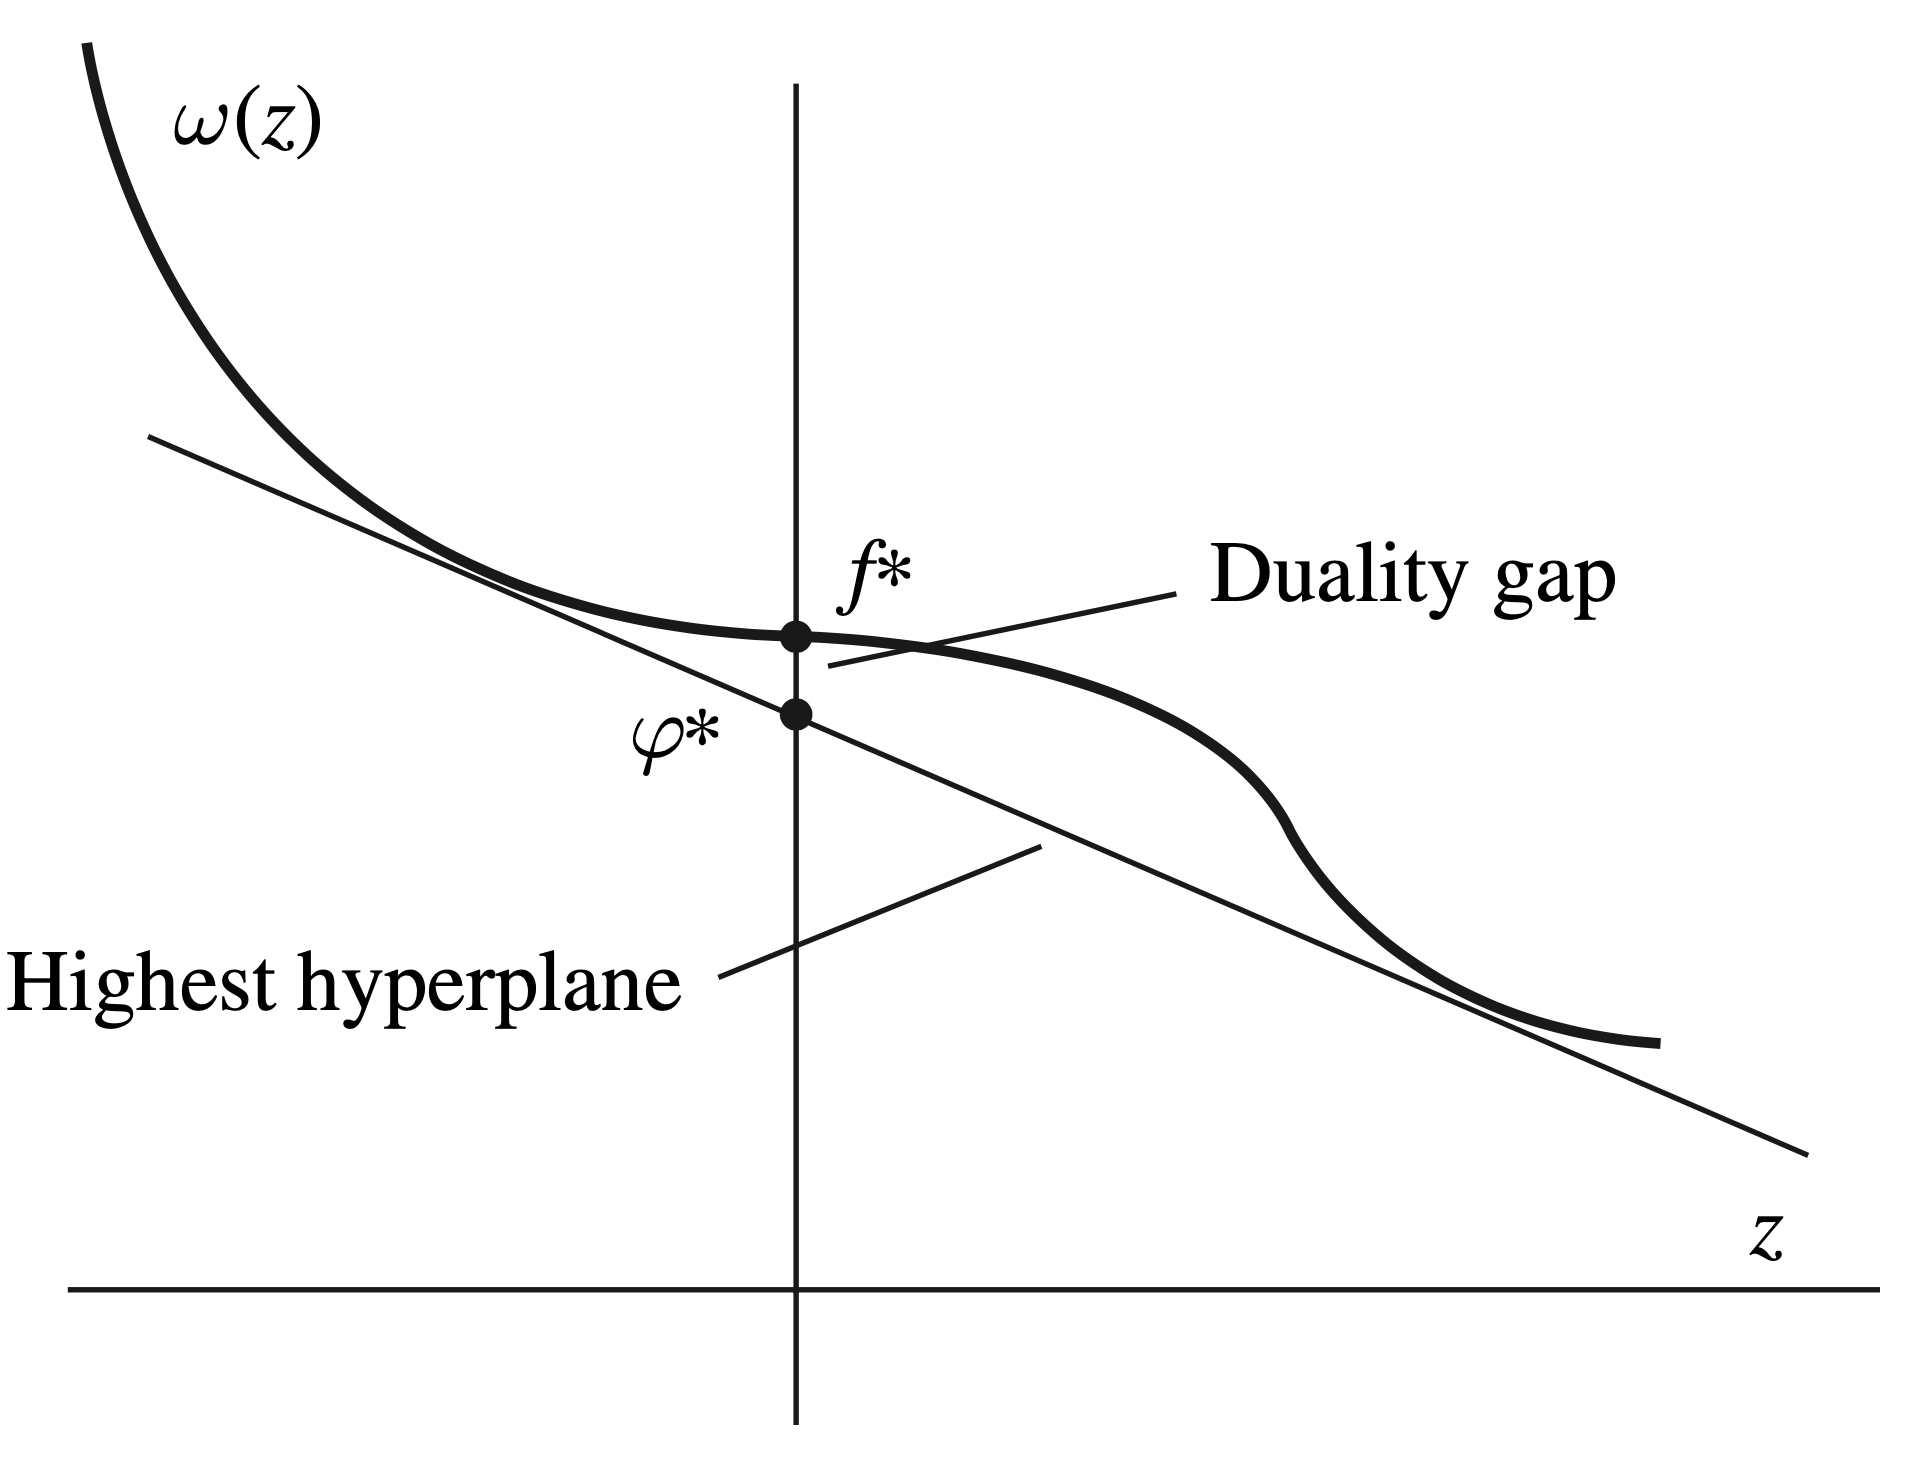
\includegraphics[scale=0.3]{Figures/duality/highest-hyperplane.png}
    \caption{对偶间距的示意图.}
    \label{fig:highest-hyperplane}
\end{figure}

由此可以得到对偶性原理:位于$\omega$之下的超平面的最大截距等于刚刚碰到$\omega$的超平面的最小截距.

如果原始函数$\omega$是凸的,那么弱对偶定理可以被加强到强对偶定理,此时$\varphi^*$和$f^*$之间不再存在对偶间距,\Cref{fig:highest-hyperplane} 变成了\Cref{fig:strong-dual}.

\begin{figure}
    \centering
    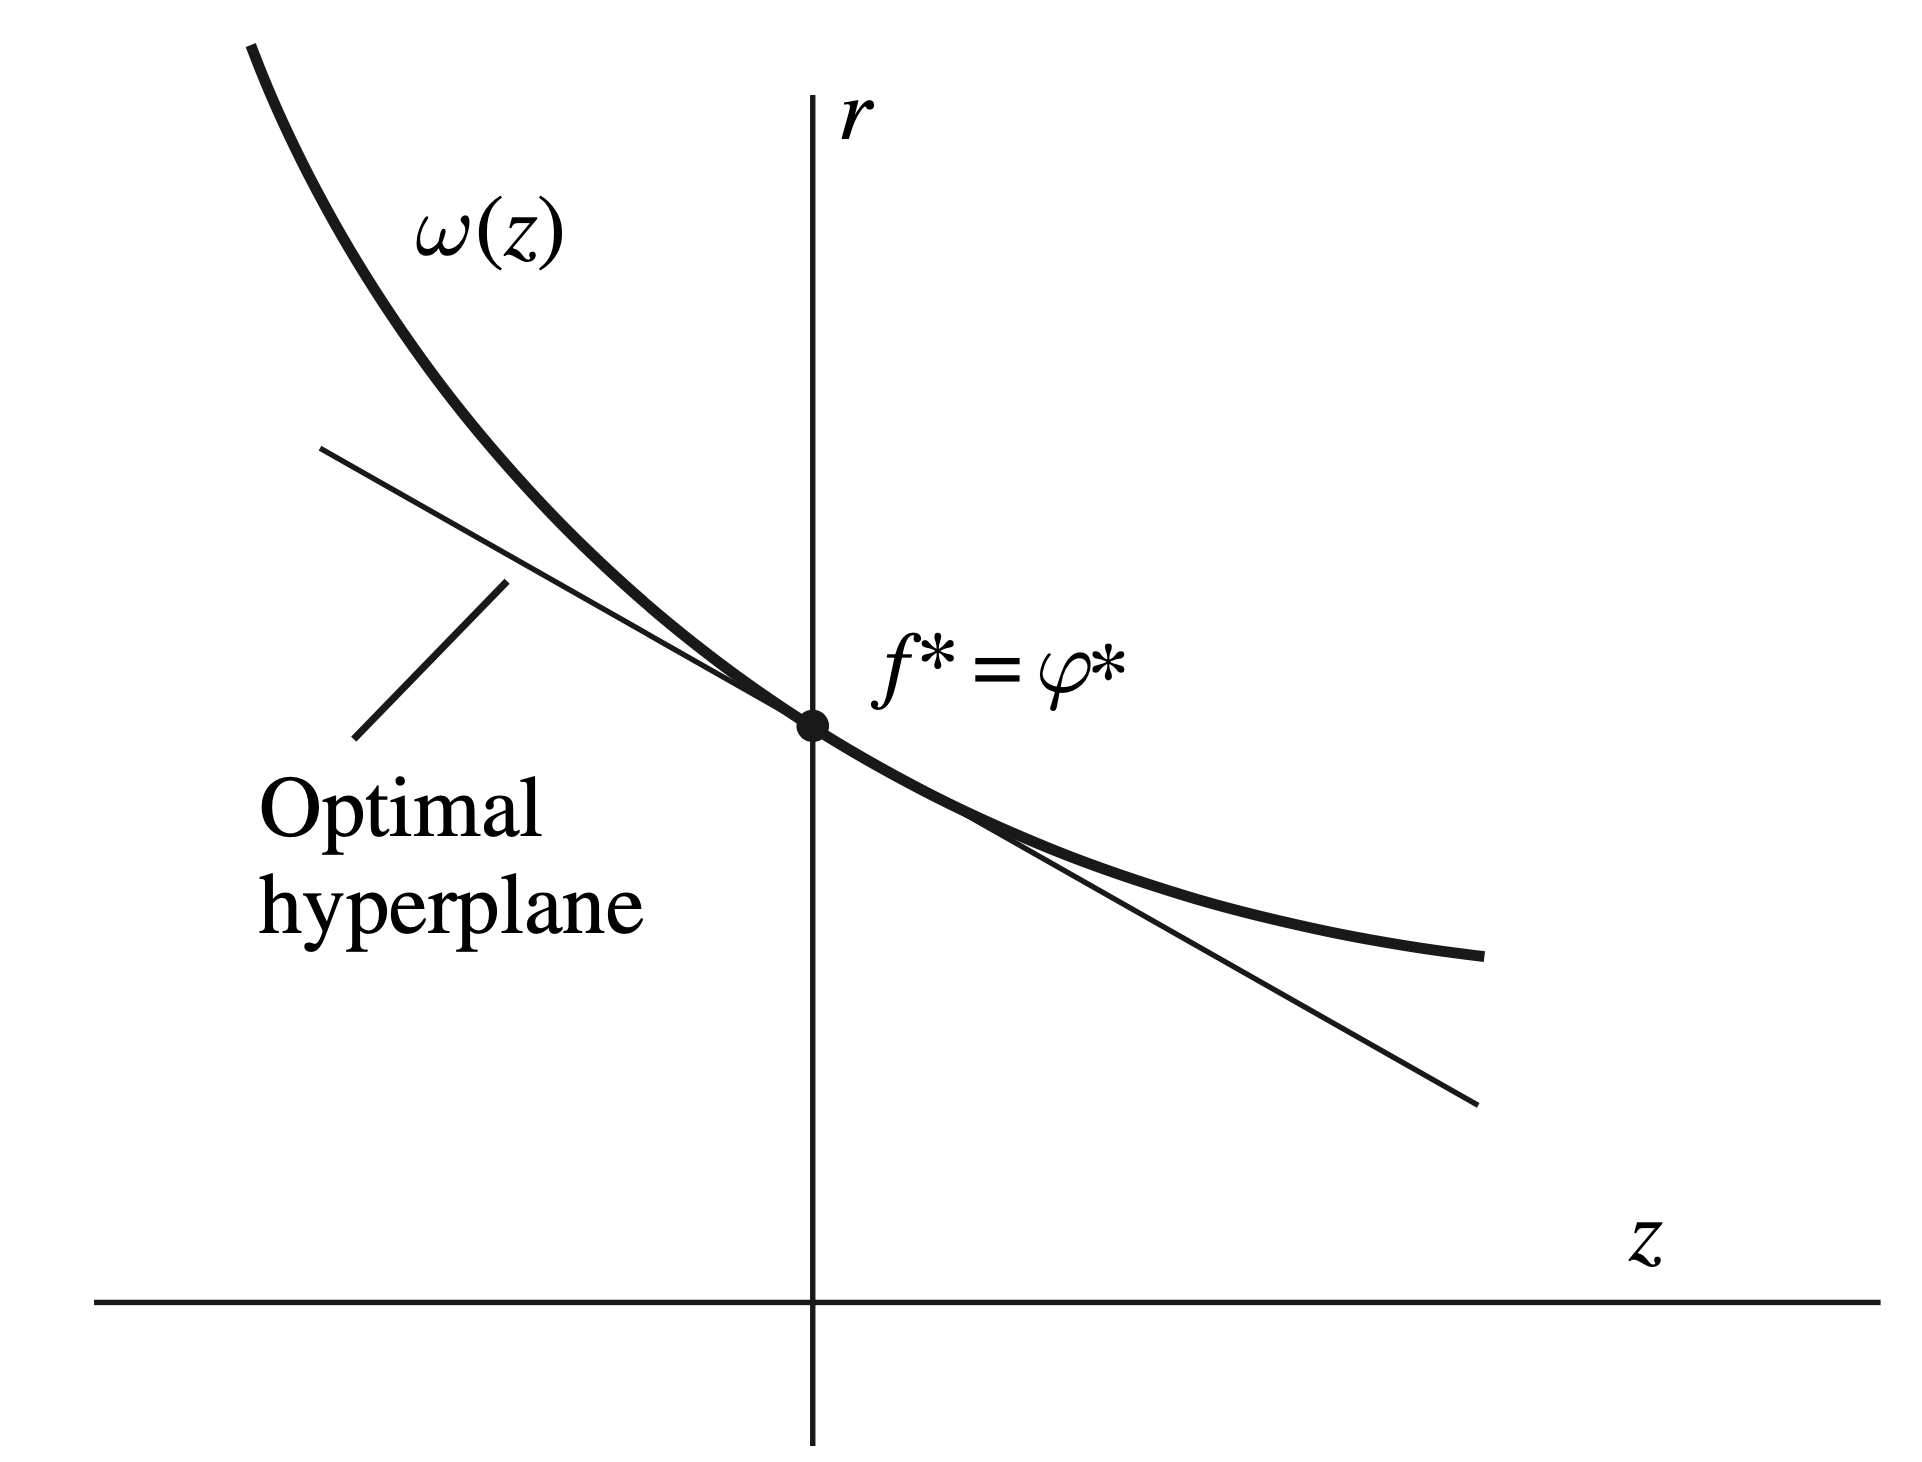
\includegraphics[scale=0.3]{Figures/duality/strong-dual.png}
    \caption{强对偶定理的示意图.}
    \label{fig:strong-dual}
\end{figure}

下面我们叙述并证明强对偶定理. 我们直接考虑一般的优化问题.
\begin{equation}
        \begin{aligned}
    \min\quad & f(x) \\
    \text{s.t.}\quad& {h(x)=0}, \\
    &g(x)\leq 0, \\
    &x\in\Omega.
    \end{aligned}\label{eq:mix-dual}
\end{equation}
其中,${h}$是$m$维仿射函数,${g}$是$p$维凸函数,$\Omega\subseteq\R^n$是凸集. 

原始函数\index{原始函数}可以写作
    \[\omega(y,z)=\inf\{f(x):\exists x\in\Omega\ h(x)=y, g(x)\leq z\}.\]
对偶函数\index{对偶函数}定义为:$$\varphi({\lambda,\mu})=\inf\{f(x)+{\lambda^\t h(x)+\mu^\t g(x):x}\in\Omega\}.$$
它的最大值记为
    $$\varphi^*=\sup\{\varphi({\lambda,\mu}):{\lambda}\in \R^m,{\mu}\in \R^p,{\mu}\geq {0}\}.$$

利用以上定义,我们可以表述强对偶定理如下:
\begin{theorem}[强对偶定理]
在问题 \eqref{eq:mix-dual} 中,假设${h}$是对于$\Omega$正规的,在可行域内$g$满足正规性条件. 假设$x^*$是问题 \eqref{eq:mix-dual} 的解,设$f(x^*)=f^*$. 那么对每个${\lambda}$和${\mu}\ge{0}$都有
$$\varphi(\lambda,\mu)\leq f^*.$$
另外,存在${\lambda,\mu\geq 0}$使得
$$\varphi({\lambda,\mu})=f^*.$$
因此$\varphi^*=f^*$. 与此同时,$\lambda,\mu$是该问题的Lagrange乘子.
\end{theorem} 

\begin{proof}
由Lagrange零阶条件定理(\Cref{thm:mix-zero-cond})可知:
    \begin{align*}
        f^*&=\min\{f(x)+{\lambda^\t h(x)+\mu^\t g(x):x}\in\Omega\}\\
        &=\varphi({\lambda,\mu})\le\varphi^*\leq f^*.
    \end{align*}
因此,$\varphi^*=f^*$,并且取等号的$\lambda,\mu$是Lagrange乘子.
\end{proof}

从对偶原理我们可以写出对偶规划的一般形式:
    \begin{align*}
    \begin{array}{cc}
        \text{原始问题} &\qquad \text{对偶问题} \\
        \begin{aligned}
            \min\quad&\omega(y,z)\\
            \text{s.t.}\quad &y=0,\\
            &z\leq 0.
        \end{aligned}&\qquad
        \begin{aligned}
            \max\quad&\varphi(\lambda,\mu)\\
            \text{s.t.}\quad &\lambda\in\R^m,\\
            &\mu\geq 0.
        \end{aligned}
    \end{array}
    \end{align*}
作为例子,下面我们给一个对偶规划的经济学解释. 

\begin{example}[线性规划的经济学解释]
\Cref{tab:cleaner} 描述了公司甲用纸浆生产抽纸的价格与存量表. 
\begin{table}
        \centering
        \begin{tabular}{c|ccc|c}
        \hline
                 & 纸浆1&纸浆2&纸浆3&售价(万元/吨) \\
                 \hline
             抽纸A  & 0.25&0.50&0.25&12 \\
             抽纸B & 0.50&0.50& &15\\
             \hline
             存量(吨)&120&150&50& \\
             \hline
        \end{tabular}
        \caption{抽纸纸浆价格存量表. }
        \label{tab:cleaner}
\end{table}

甲用3种纸浆混合成2种抽纸. 2种抽纸应该如何配制,使总价值最大?

设抽纸A和B分别配制$x_1$和$x_2$,我们可以把甲的目标写成一个规划问题:
\begin{align*}
\begin{array}{lrcl}
\max\quad&\multicolumn{3}{l}{z=12x_1+15x_2}\\
\text{s.t.}\quad&0.25x_1+0.50x_2&\le&120,\\
&0.50x_1+0.50x_2&\le&150,\\
&0.25x_1&\le& 50,\\
&x_1&\ge& 0,\\
&x_2&\ge& 0.
\end{array}
\end{align*}

现在有一个公司乙需要这3种纸浆,打算向甲购买,应付出多少钱?

乙向甲购买3种纸浆,出价分别为每吨$y_1,y_2,y_3$万元. 希望总价格尽量小,但不能低于甲用纸浆生产抽纸所产生的价值,因此写出规划问题为:
\[
 \begin{array}{lrcl}
\min\quad&\multicolumn{3}{l}{w=120y_1+150y_2+50y_3} \\
\text{s.t.}\quad& 0.25y_1+0.50y_2+0.25y_3&\ge&12,\\
&0.50y_1+0.50y_2&\ge&15,\\
&y_1&\ge&0,\\
&y_2&\ge&0,\\
&y_3&\ge&0.
 \end{array}
\]
注意到,以上两个规划问题恰好互为对偶问题.
\end{example}

\section{应用:支持向量机(SVM)}\index{支持向量机}\index{SVM}

作为前面极值必要条件的一个具体应用,我们考虑一个经典的机器学习分类器:\emph{支持向量机}(SVM). 

考虑二分类问题,输入$x\in \R^n$,函数$f$输出一个$\{-1,1\}$中的值. 二分类问题的学习问题指的是给定训练集$\{(x_i,y_i)\}_{i=1}^N$,找到$f$使得$f(x_i)=y_i$. 假设训练集是线性可分的,例如,存在某个$w\in \R^n$和$b\in \R$使得
    $$f(x)=\begin{cases}
		1,& w^\t x+b>0,\\
		-1, &w^\t x+b<0.
	\end{cases}$$

学习问题的首要目标是找到正确的以及最优的$w$和$b$. 本质上说,这就是一个\emph{找分离超平面}\index{分离超平面}的过程. 那么,什么才叫最优呢?从几何视角来看,一个自然的想法是最大化\emph{分离距离}\index{分离距离},即训练集中所有点到分离超平面的距离和的最小值,见\Cref{fig:svm}.
\begin{figure}
    \centering
    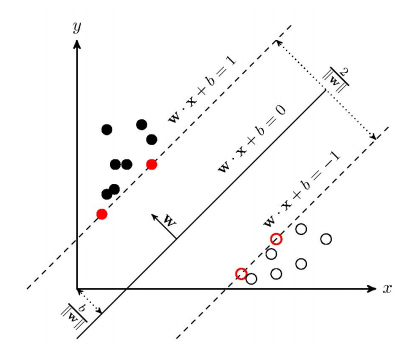
\includegraphics[scale=0.8]{Figures/duality/svm.png}
    \caption{分离距离示意图.}
    \label{fig:svm}
\end{figure}

采样点$x_i$到分离超平面的归一化距离为
    $$\gamma_i=y_i\left(\left(\frac{w}{\norm{w}_2}\right)^\t x+\frac{b}{\norm{w}_2}\right).$$
$\gamma=\min_i\gamma_i$是最小的归一化距离. 于是我们的任务变成了最大化$\gamma$. 等价地,我们求解如下优化问题
\begin{align*}
    \max_{w,b}\quad&\gamma \\
    \text{s.t.}\quad&\gamma\le\gamma_i,\quad i=1,2,\dots,N.
\end{align*}

$\gamma\le\gamma_i$等价于$$y_i\left(\left(\frac{w}{\gamma\norm{w}_2}\right)^\t x+\frac{b}{\gamma\norm{w}_2}\right)\geq 1.$$
简洁起见,把$w$替换成$\frac{w}{\gamma\norm{w}_2}$,把$b$替换成$\frac{b}{\gamma\norm{w}_2}$,我们有$$y_i(w^\t x+b)\geq 1.$$
那么最大化$\gamma=\frac{1}{\norm{w}_2}$等价于最小化$\norm{w}_2^2$. 

我们得到以下凸规划问题:
\begin{align*}
    \min_{w,b}\quad&\frac{1}{2}\|w\|_2^2\\
    \text{s.t. }\quad &y_i(w^\t x_i+b)\geq 1,\quad i=1,2,\cdots, N.
\end{align*}

如何解决这个问题?利用上面的对偶理论,我们有如下步骤:
\begin{itemize}
    \item 第一步,用Lagrange乘子法,转化成Lagrange问题(min-max).
    \item 第二步,写出对偶问题(max-min),验证强对偶定理的正规性条件,于是只需要求解对偶规划.
    \item 第三步,写出KKT条件,将对偶规划解为一个二次规划(min) ,用优化算法求解二次规划.
\end{itemize}